%% ======================================================================
\section{\CLvs}
\label{sec:covVecs}

The recent progress
in numerical methods to calculate \emph{\cLv}s\rf{GiChLiPo12, KuPa12}
has motivated us to explore an inertial manifold by
\cLvs\ locally through a statistical study of the tangency among
\cLvs\rf{YaTaGiChRa08} and
difference vector projection\rf{YaRa11}. The number of the \cLvs\ needed
for locally spanning the inertial manifold is
regarded as the dimension of an inertial manifold. The key observation
in this study is that tangent space can be decomposed into an
entangled ``physical'' subspace and its complement, a contracting
disentangled subspace.
The latter plays no role in the longtime behavior
on the inertial manifold.

In this section, we will introduce covariant vectors (often called
``covariant Lyapunov vectors'' in the literature\rf{GiChLiPo12,
ginelli-2007-99}) associated with \po s and ergodic orbits. The
general setup is that we have an autonomous continuous flow described by
\begin{equation}
  \label{eq:flow}
  \dot{\ssp} = \vel(\ssp) \,, \quad \ssp(x, t) \in \reals^n
  \,.
\end{equation}
The corresponding time-forward trajectory starting from $\ssp_0$ is
$\ssp(t)=\flow{t}{\ssp_0}$.
In the linear approximation, the equation that governs
the deformation of an infinitesimal neighborhood of
$\ssp(t)$ (dynamics in tangent space) is
\begin{equation}
  \label{eq:stab}
  \frac{d}{dt}\delta \ssp = A \delta\ssp \,, \quad
  A = \frac{\partial \vel}{\partial \ssp}
  \,.
\end{equation}
Matrix $A$ is called the stability matrix of the flow. It describes the
rates of instantaneous expansion/contraction and shearing in the tangent space.
The \JacobianM\ of the flow transports linear perturbation along the orbit:
\begin{equation}
  \label{eq:jacob}
  \delta \ssp(\ssp, t)=\jMps^\zeit(\ssp_0, 0)\,\delta \ssp(\ssp_0, 0)
\end{equation}
Here we make it explicit that the infinitesimal deformation
$\delta \ssp$ depends on both
the orbit and time. The \JacobianM\ is obtained by integrating equation
\begin{equation}
  \label{eq:tangentDynamics}
  \frac{d}{dt}\jMps = A \jMps \,, \quad
  J_0 = I
  \,.
\end{equation}
\JacobianM\ satisfies the semi-group multiplicative property (chain rule)
along an orbit,
\begin{equation}
  \jMps^{\zeit-\zeit_{0}}(\ssp(\zeit_{0}) ,\zeit_{0})
  =
  \jMps^{\zeit-\zeit_{1}}(\ssp(\zeit_{1}),\zeit_{1})
  \jMps^{\zeit_{1}-\zeit_{0}}(\ssp(\zeit_{0}),\zeit_{0})
  \,.
  \label{eq:xjacobian}
\end{equation}


\subsection{\Fv s}
\label{sect:LinStab}

For a point
$\ssp(\zeit)$ on a \po\ $p$ of period \period{p},
\begin{equation}
  \label{eq:fm}
  \jMps_p=\jMps^{\period{p}}(\ssp, \zeit)
\end{equation}
is called the Floquet matrix
(monodromy matrix), and its
eigenvalues the Floquet multipliers $\ExpaEig_{j}$.
The $j$th Floquet multiplier is a dimensionless ratio of
the final/initial
deformation along the $j$th eigendirection. It is an intrinsic, local
property of a smooth flow, invariant under all smooth coordinate
transformations. The associated
\Fv s $\jEigvec[j](\ssp)$,
\begin{equation}
  \label{eq:fv}
  \jMps_p\,\jEigvec[j]=\ExpaEig_{j}\jEigvec[j]
\end{equation} define the invariant
directions of the tangent space at periodic point
$\ssp(\zeit)\in p$. Evolving a small initial perturbation aligned with
an expanding Floquet direction will generate the corresponding
unstable manifold along
the \po. Written in exponential form
\[
  \ExpaEig_{j} = \exp(\period{p}\Lyap^{(j)}_p)\
  = \exp(\period{p}\eigRe[j] + i\theta_j)
  \,,
\]
where $\Lyap^{(j)}_p$\footnote{Here, subscript $p$ emphasizes
  that it is
  associated with a \po\ so as to distinguish it
  with the Lyapunov exponents defined in
  the next section.} are the
Floquet exponents.
Floquet multipliers are either real,
$\theta_j = 0, \pi$, or form
complex pairs, $\{\ExpaEig_{j},\ExpaEig_{j+1}\} =
\{|\ExpaEig_{j}|\exp(i\theta_j),|\ExpaEig_{j}|\exp(-i\theta_j)\}$, $0
<\theta_j <\pi$. The real parts of the
Floquet exponents
\begin{equation}
  \label{eq:fe}
  \eigRe[j] = (\ln|\ExpaEig_{j}|)/\period{p}
\end{equation}
describe the mean contraction or
expansion rates per one period of the orbit.
Appendix \ref{sec:floq} talks about the form of the \JacobianM\ of
a general linear flow with periodic coefficients.

\subsection{\CLv s}

For a \po, the Jacobian matrix of $n$ periods is the $n$th power of the Jacobian
corresponding to a single period. However, for an ergodic orbit, there is no
such simple relation. Integrating \JacobianM\ by
\refeq{eq:tangentDynamics} cannot be avoided for studying asymptotic stability of this
orbit. However, similar to \Fv s of a \po, a set of \cLvs\
exists for an ergodic orbit.
\emph{Multiplicative ergodic theorem}\rf{lyaos,ruelle79} says that the forward and backward
Oseledets matrices
\begin{equation}
  \Xi^{\pm}(\ssp) :=\lim_{t\to\pm\infty}[J^t(\ssp)^\top J^{t}(\ssp)]^{1/2t}
  \label{eq:oseledets}
\end{equation}
both exist for an invertible dynamical system equipped with an invariant measure.
Their eigenvalues are
$e^{\Lyap^{+}_1(\ssp)}<\cdots<e^{\Lyap^{+}_s(\ssp)}$,
and $e^{\Lyap^{-}_1(\ssp)}>\cdots>e^{\Lyap^{-}_s(\ssp)}$ respectively,
with $\Lyap^{\pm}_i(\ssp)$ the
Lyapunov exponents (characteristic exponents) and $s$
the total number of distinct exponents ($s\le n$). For an ergodic system,
Lyapunov exponents are the same almost everywhere, and
\begin{equation}
  \label{eq:lyap}
  \Lyap^{+}_i(\ssp)=-\Lyap^{-}_{i}(\ssp)=\Lyap_i
\end{equation}
The corresponding eigenspaces
$U^\pm_1(\ssp), \cdots, U^\pm_s(\ssp)$
can be used to construct the forward and backward invariant subspaces:
\begin{align*}
  V^+_i(\ssp) & = U^+_1(\ssp) \oplus \cdots \oplus U^+_i(\ssp) \\
  V^-_i(\ssp) & = U^-_i(\ssp) \oplus \cdots \oplus U^-_{s}(\ssp)
  \,.
\end{align*}
So the intersections
\begin{equation}
  \label{eq:inter}
  W_i(\ssp)=V^+_i(\ssp)\cap V^-_i(\ssp)
\end{equation}
are dynamically
forward and backward invariant: $J^{\pm t}(\ssp)W_i(\ssp) \to W_i(\flow{\pm t}{\ssp})$,
$i = 1, 2,\cdots,s$. \refeq{eq:inter} is called the Oseledets splitting.
The expansion rate in the invariant subspace $W_i(\ssp)$ is given
by the corresponding Lyapunov exponent,
\begin{equation}
  \label{eq:lyapunov}
  \lim_{t\to\pm\infty}\frac{1}{|t|}\ln\norm{J^t(\ssp)v}
  =\lim_{t\to\pm\infty}\frac{1}{|t|}\ln\norm{[J^t(\ssp)^\top J^t(\ssp)]^{1/2}v}
  = \pm\Lyap_i
  \,,\quad v\in W_i(\ssp)
  \,.
\end{equation}
If a Lyapunov exponent is nondegenerate, the corresponding
subspace $W_i(\ssp)$ reduces to a vector, called \emph{\cLv}.
For \po s, these $\Lyap_i$
(evaluated numerically as $\zeit\to\infty$ limits of many repeats of the
prime period $\period{}$) coincide with the real parts of Floquet exponents
\refeq{eq:fe}. Subspace $W_i(\ssp)$ coincides with
a \Fv, or, if there is degeneracy, a subspace
spanned by \Fv s.

The reorthonormalization procedure
formulated by Benettin \etal\rf{bene80a}
is
the standard way to calculate the full spectrum of Lyapunov exponents,
and it is shown\rf{ErshPot98}
that the orthogonal vectors produced at the end of
this procedure converge to $U_i^{-}(\ssp)$, eigenvectors of $\Xi^{-}(\ssp)$, called
the Gram-Schmidt (GS) vectors (or backward Lyapunov vectors).
Based on this technique,
Wolf \etal\rf{WoSa07} and
Ginelli \etal\rf{GiChLiPo12, ginelli-2007-99}
independently invented distinct methods to recover \cLv s
from GS vectors. Here, we should emphasize that GS vectors are
not invariant. Except for the leading one, all of them depend on
the specific inner product imposed by the dynamics. Also, the local expansion
rates of \cLv s are not
identical to the local expansion rates of GS vectors. Specifically for
\po s, \Fv s depend on no norm and map forward and
backward as $\jEigvec[j] \to \jMps\,\jEigvec[j]$ under time evolution.
In contrast, the linearized dynamics does not transport GS vectors into
the tangent space computed further downstream. For a detailed
comparison, please see\rf{KuPa12, YaRa10}.

\subsection{\CLv s algorithm}
\label{subsec:clvs}

\begin{figure}
  \centering
  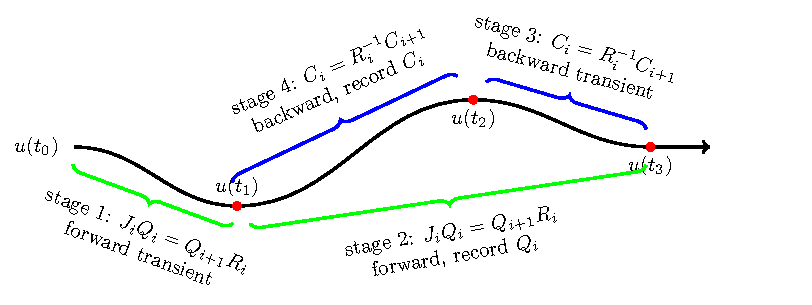
\includegraphics[width=1\textwidth]{cLv}
  \caption[Four stages of \cLv\ algorithm]
  {Four stages of \cLv\ algorithm.
    The black line is a part of
    a long ergodic trajectory.}
  \label{fig:CLV}
\end{figure}
Here we briefly introduce the method used by
Ginelli \etal\rf{GiChLiPo12, ginelli-2007-99}
to extract
\cLvs\ from GS vectors. The setup is the same as computing Lyapunov
exponents. We follow a long ergodic trajectory and integrate
the linearized dynamics in tangent space \eqref{eq:tangentDynamics}
with orthonormalization regularly, shown as the first two stages in
\reffig{fig:CLV}.
Here, $J_i$ is the short-time \JacobianM,
and $Q_{i+1}R_i$ is the $QR$ decomposition of $J_iQ_i$.
We use the new generated orthonormal matrix $Q_{i+1}$ as the initial condition
for the next short-time integration of \eqref{eq:tangentDynamics}.
Therefore, if we choose an appropriate time length of each integration segment,
we can effectively avoid numerical instability by repeated $QR$ decomposition.
Set the initial
deformation matrix $Q_0 = I$, then after $n$ steps in stage 1, we obtain
\[
  J_{n-1}\cdots J_0 = Q_n R_n\cdots R_0
  \,.
\]
The diagonal elements
of upper-triangular
matrices $R_i$ store local
Lyapunov exponents, longtime average of which gives the Lyapunov
exponents of this system. In stage 1, we discard all these
upper-triangular matrices $R_i$. We assume that $Q_i$ converges
to the GS vectors after stage 1, and start to record $R_i$ in
stage 2. Since the first $m$ GS vectors span the same subspace as the
first $m$ \cLv s, which means
\begin{equation}
  \label{eq:cv_T}
  T_i = Q_iC_i
  \,.
\end{equation}
Here $T_i = [W_1, W_2,\cdots, W_n]$ refers to the matrix whose columns
are \cLv s at step $i$ of this algorithm.
$C_i$ is an upper-triangular matrix, giving the expansion
coefficients of \cLv s in the GS basis. Since $J_{i-1}Q_{i-1}=Q_iR_i$,
we have $T_i = J_{i-1} Q_{i-1} R^{-1}_{i}C_i$.
Also since $T_{i-1} = Q_{i-1}C_{i-1}$, we get
\begin{equation}
  \label{eq:cv_T2}
  T_{i} = J_{i-1}T_{i-1}C_{i-1}^{-1}R^{-1}_{i}C_i
\end{equation}
Since $T_i$ is invariant in the
tangent space, namely, $J_{i-1}T_{i-1}=T_iD_i$ with
$D_i$ a diagonal matrix concerning the stretching and
contraction of \cLv s. Substitute it into \refeq{eq:cv_T2}, we get
$I = D_iC_{i-1}^{-1}R^{-1}_{i}C_i$. Therefore,
we obtain the backward dynamics of
matrix $C_i$ :
\begin{equation}
  \label{eq:cv_back}
  C_{i-1} = R^{-1}_{i} C_iD_i
\end{equation}
Numerically, $D_i$ is
not formed explicitly since it is only a normalization factor.
Ginelli \etal\rf{GiChLiPo12, ginelli-2007-99}  cleverly uncover
this backward dynamics and show that $C_i$ converges after a sufficient
number of iterations (stage 3 in \reffig{fig:CLV}). We choose an arbitrary
upper-triangular matrix as the initial input for the backward iteration
\refeq{eq:cv_back}, $R_i$ are those upper-triangular matrices recorded during
stage 2, and $R_i^{-1}$ are also upper-triangular. The product of two
upper-triangular matrices is still upper-triangular. Thus, backward iteration
\refeq{eq:cv_back} guarantees that $C_i$ are all upper-triangular.
This process
is continued in stage 4 in \reffig{fig:CLV}, and $C_i$ are recorded
at this stage.
For trajectory segment $\ssp(t_1)$ to $\ssp(t_2)$ in \reffig{fig:CLV},
we have the converged GS basis $Q_i$ and the converged $C_i$,
then by \refeq{eq:cv_T},
we obtain the \cLv s corresponding to this segment.

\CLv\ algorithm is invented to stratify the tangent spaces along
an ergodic trajectory, so it is hard to observe
degeneracy numerically. However, for \po s, it is
possible that some \Fv s form conjugate complex pairs.
When this algorithm is applied to \po s, it is reduced
to a combination of simultaneous iteration and inverse
power iteration;
consequently, complex conjugate pairs cannot be told apart.
This
means that we need to pay attention to the two\dmn\ rotation
when checking the convergence of each stage in \reffig{fig:CLV}.
As is shown in \refchap{chap:ped}, a complex conjugate pair
of \Fv s can be extracted from a converged
two\dmn\ subspace.

%======================================================================
\subsection{\Psd\ algorithm}
\label{subsec:psd}

\begin{figure}
  \centering
  \begin{align*}
    \small
    \setlength\arraycolsep{1pt}
    \renewcommand{\arraystretch}{0.7}
    \begin{bmatrix}
      x & x & x & x & x & x \\
      x & x & x & x & x & x \\
      x & x & x & x & x & x \\
      x & x & x & x & x & x \\
      x & x & x & x & x & x \\
      x & x & x & x & x & x \\
    \end{bmatrix}
    \begin{bmatrix}
      x & x & x & x & x & x \\
      x & x & x & x & x & x \\
      x & x & x & x & x & x \\
      x & x & x & x & x & x \\
      x & x & x & x & x & x \\
      x & x & x & x & x & x \\
    \end{bmatrix}
    \begin{bmatrix}
      x & x & x & x & x & x \\
      x & x & x & x & x & x \\
      x & x & x & x & x & x \\
      x & x & x & x & x & x \\
      x & x & x & x & x & x \\
      x & x & x & x & x & x \\
    \end{bmatrix}
        & \xrightarrow{\normalsize \text{stage 1}}
        % & \overset{\text{\normalsize stage 1}}{\large \to}
            \small
            \setlength\arraycolsep{1pt}
            \renewcommand{\arraystretch}{0.7}
            \begin{bmatrix}
              x & x & x & x & x & x \\
              x & x & x & x & x & x \\
              & x & x & x & x & x \\
              &   & x & x & x & x \\
              &   &   & x & x & x \\
              &   &   &   & x & x \\
            \end{bmatrix}
    \begin{bmatrix}
      x & x & x & x & x & x \\
      & x & x & x & x & x \\
      &   & x & x & x & x \\
      &   &   & x & x & x \\
      &   &   &   & x & x \\
      &   &   &   &   & x \\
    \end{bmatrix}
    \begin{bmatrix}
      x & x & x & x & x & x \\
      & x & x & x & x & x \\
      &   & x & x & x & x \\
      &   &   & x & x & x \\
      &   &   &   & x & x \\
      &   &   &   &   & x \\
    \end{bmatrix} \\
        & \xrightarrow{\normalsize \text{stage 2}}
          \small
          \setlength\arraycolsep{1pt}
          \renewcommand{\arraystretch}{0.7}
          \begin{bmatrix}
            x & x & x & x & x & x \\
            & x & x & x & x & x \\
            & x & x & x & x & x \\
            &   &   & x & x & x \\
            &   &   &   & x & x \\
            &   &   &   &   & x \\
          \end{bmatrix}
    \begin{bmatrix}
      x & x & x & x & x & x \\
      & x & x & x & x & x \\
      &   & x & x & x & x \\
      &   &   & x & x & x \\
      &   &   &   & x & x \\
      &   &   &   &   & x \\
    \end{bmatrix}
    \begin{bmatrix}
      x & x & x & x & x & x \\
      & x & x & x & x & x \\
      &   & x & x & x & x \\
      &   &   & x & x & x \\
      &   &   &   & x & x \\
      &   &   &   &   & x \\
    \end{bmatrix}
  \end{align*}
  \caption[Two stages of \psd\ algorithm ]
  {Two stages of \psd\ algorithm illustrated by
    three $[6\!\times\! 6]$ matrices. Empty locations are zeros.}
  \label{fig:PSD}
\end{figure}
Here, we review another algorithm related to our work.
The double-implicit-shift QR algorithm\rf{Trefethen97,DSWatkins}
is the standard way
of solving the eigen-problem of a single matrix in many numerical packages,
such as the
\texttt{eig()} function in Matlab.
Bojanczyk \etal\rf{Bojanczyk92theperiodic}
extend this
idea to obtain \emph{\psd} of the product of a sequence of matrices. Later on,
Kurt Lust\rf{Lust01} describes the implementation details and provides
the corresponding
Fortran code.
On the other hand, by use of the chain rule \eqref{eq:xjacobian}, the
\JacobianM\ can be decomposed into a product of short-time
Jacobians with the same dimension. Therefore, \psd\ is well suited for computing
Floquet exponents.

As illustrated in \reffig{fig:PSD}, \psd\ proceeds in two stages.
First, the sequence
of matrices is transformed to the \emph{Hessenberg-Triangular} form,
one of which has upper-Hessenberg form while the others
are upper-triangular,
by a series of Householder transformations\rf{Trefethen97}.
The second stage tries to diminish the sub-diagonal components of
the Hessenberg matrix until it becomes quasi-upper-triangular,
that is, there are some
$[2\!\times\! 2]$ blocks on the diagonal corresponding to
complex eigenvalues. The eigenvalues of the matrix product are
given by the products of all individual matrices' diagonal elements.
However, \psd\ is not sufficient for extracting eigenvectors, except the leading one.
Kurt Lust\rf{Lust01} claims to formulate the corresponding
\Fv\ algorithm, but to
the best of our knowledge, such an algorithm is not present in the literature.
Fortunately, Granat \etal\rf{GranatK06} have proposed a method to reorder diagonal
elements
after \psd. This provides an elegant way to compute \Fv s as we will see in
\refchap{chap:ped}.
